\subsection{Data Flow}

\subsubsection{Input and Processing}
Multiple formats can be processed using the command line tool that has been developed during this project. Initially only TCPdump was considered, the tool took input in the form of binary PCAP files, this was then extended to allow syslog formats to be used as input. The output produced is in an identical format regardless of the input type. Data flow for the two input types is similar and detailed in figure \ref{fig:df_dia}.\newline
\begin{figure}[h]
    \centering
    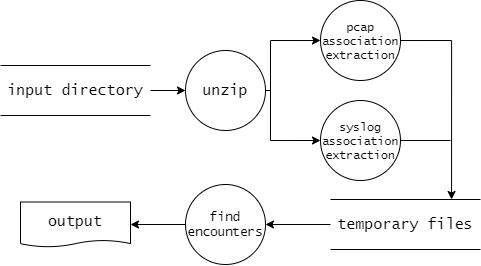
\includegraphics[width=0.7\textwidth]{df_diagram.png}
    \caption{This figure shows the flow of data through the system, including temporary file stores and input/output to each processing stage.}
    \label{fig:df_dia}
\end{figure}

The first stage of processing is to extract associations between devices and access points from the raw input. These associations will later be compared with each other to determine encounters between devices, these comparisons are expensive and so it is important that as much information as possible is removed before they are made. The intermediate format used to store association information is  a comma separated value file with fields of source id, destination id, start time, end time, and AP flag. The AP flag is set to 1 only if the destination address of the association can be identified as an access point. Methods used to identify access points are discussed later in this report.

TCPdump output PCAP files are very strictly structured. This allows for them to be processed without any additional information from the user. However the initial parsing is expensive with respect to time since so much information is contained within them. In comparison to this, syslog files are relatively quick to parse for associations, but the user must include a configuration file to specify the format used. Details such as defining features of association end points and the format of device identification values need to be given to the tool before it can extract associations. The expected format of a configuration file for use with syslog is detailed in figure \ref{fig:JSON_config}.\newline

\begin{figure}[h]
    \centering
    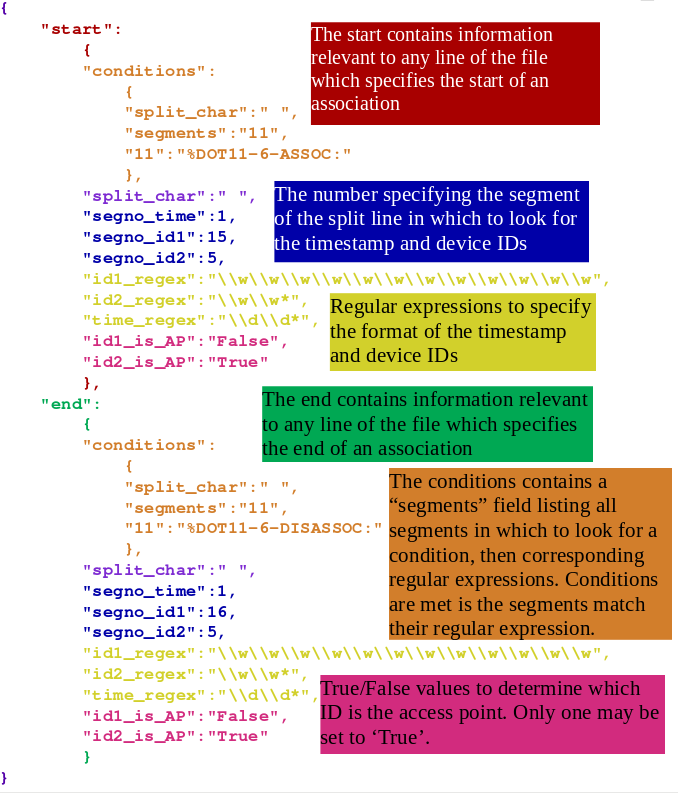
\includegraphics[width=0.9\textwidth]{JSON_config.png}
    \caption{This figure shows a configuration file used for the processing of the dartmouth/campus Aruba syslog files. The fields have been colour coded for readability and descriptions of the fields have been given. The colour does not reflect any formatting of the actual configuration file.}
    \label{fig:JSON_config}
\end{figure}

Tying together the components of this data flow is a BASH script. Temporary files are used for storing associations in the intermediate stages, these files are then read by the MatLab script which compares associations to find encounters. A final output file is then given as a comma separated values file. 
% Optional levels of abstraction??

% explain fields chosen
%   - how is encounter data used in external studies?
% Data flow diagrams
% BASH scripting

\subsubsection{Summary Output}
The final output specifies the endpoints of encounters, the average time of encounters between the given end points, and the number of encounters found between the given end points. Only one entry in the CSV file is present for each unordered pair of end points. A small section of an output summary is shown in figure \ref{fig:output}, it has been colour coded for ease of reading.\newline
\begin{figure}[h]
    \centering
    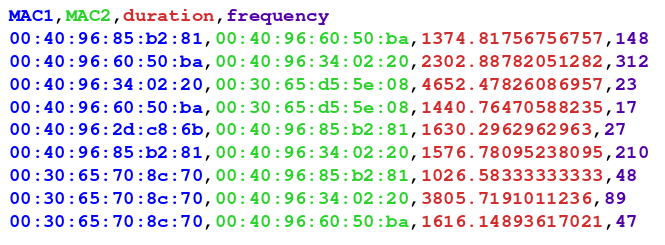
\includegraphics[width=0.8\textwidth]{Output_Example_Coloured.png}
    \caption{This figure shows a small section of an output file produced by the summarisation tool developed during this project. The columns have been colour coded for readability, but this does not reflect any formatting of the output CSV.}
    \label{fig:output}
\end{figure}

The data sets which I am using in this project have in the past frequently been used for research into mobility and encounter patterns between users \cite{Scellato2011} \cite{Xiao2014} \cite{Hsu2010} \cite{Musolesi2009} \cite{Kosta2014} \cite{Kumar2009} \cite{Wei2013}. To maximise the usefulness of this project it is intended that the output from this  summarisation tool will be able to help in identifying whether a dataset is appropriate for use in mobility research, and to provide a standard format between multiple input formats which can be used for onward processing.

\subsection{Associations} 
In this project two identifiable devices are considered to be associated with each other for any period of time during which they are exchanging data. Although in this context only associations between one mobile node and one access point are relevant, a device might only be identified as an access point after several packets have been exchanged with it. It is therefore important that all associations are detected and recorded until a full list of access points is available.
%(what? why?)
\subsubsection{Identifying Access Points}
Access points need to be determined as only the associations with access points are needed in the later stage of this processing. Access points may be identified from tcpdump traces by reading the flags in the TCP header of the packets sent to them. If the SYN control flag of TCP packets is checked, when it is set the destination of the packet can be determined to be an access point. Once a packet is identified as an access point a flag is set by it in the intermediate temporary associations CSV file. This flag is used in later processing to remove all irrelevant associations from the data and to create a record of all detected access points in the network.\\\\
This method of detecting access points means that access points which do not exchange TCP data with any mobile nodes will not be detected, and therefore encounters which occur through them will not be recorded. It is unlikely for a network trace running over a significant period of time that an access point will associate with multiple devices and yet not transfer any TCP packets with them.\\\\
When parsing syslog files the location and format of the access points identifications should be specified in the configuration file. As all association and disassociation messages in a syslog file should contain an access point, all lines in the intermediate temporary associations CSV file created from a syslog input will be set as true. Despite this potentially seeming to be a waste of time to set all flags to true, it is necessary to maintain the intermediate format so that the next stage of processing can be completed using the same method regardless of initial input format.
Some input files showed hundreds of access points being detected. This is likely due to each physical access point having many separate MAC addresses with which it will communicate. There is no way to identify which addresses correspond to the same physical access point without a record to match them against. Since such a record is not available for the CRAWDAD dartmouth/campus data (and likely wouldn't be immediately available for most network traces someone might want to use with this summarisation tool) the decision has been made to only consider an encounter to have taken place is both mobile devices are connected to the same access point MAC address. This is similar to saying that each MAC address being used by a physical access point has been considered as a separate device.
\subsubsection{Initiation} 
% (what? why?)
A design decision needed to be made regarding the conditions that would specify the beginning of an association between two devices. This is an important part of the design of this system since it defines the meaning of an association, and therefore the meaning of an encounter in the final output of the system.\\\\
Identifying association request packets could be used as a method of identifying the beginning of associations. However it has been found during development that often two devices are in contact and transmit data between themselves without ever sending an association request packet. Since an association is open during the period of time which two devices are communicating for, a simplistic way of finding the start of an association may be the timestamp of the first packet transmitted between two identifiable devices.\\\\
My decision on this is that with a tcpdump input, the initiation of an association is triggered by a packet being transmitted between two devices which do not currently have an ongoing association. While an association is ongoing a transmission between the endpoints will not trigger a new association. If only one packet is transmitted between the endpoints within the timeout period it is not considered as an association. This is because it may have been a message sent to an unavailable destination, and in such a situation no contact is made between the source and destination devices.\\\\
When a syslog file is used as input the configuration file should contain conditions for a message to define the start of an association. These condition will have to be checked against each line in the syslog file to find the beginning of each association. The endpoints of the association should also have their identifications location and format within the line described in the configuration file. In the case that a configuration file specifies conditions which are ambiguous (for instance causing multiple matches for a devices identification within the line) or too strict (for instance not finding any association start messages or not being able to identify any device identifications which match the conditions given int he configuration file) then the user should be warned so that they can update the configuration file if necessary.
% options
% decision

\subsubsection{End of Association} 
% (what? why?)
In some cases a specific message or packet type may be found which determines that a device has moved out of range of an access point. This would mean that the association between that device and access point has come to an end. However, in the pcap traces which I have been focusing on it seems common that the end of an association is not explicitly signalled in the trace. In these cases another method of detecting an appropriate time for ending an association is needed. \\\\
Research into work already done with the CRAWDAD data \cite{kotz2002} \cite{henderson2004} shows that a timeout of thirty minutes has previously been considered to be adequate for determining the end of a session, leading to a deauthentication of the device. This timeout length will therefore be use in this project to catch the end of associations when no explicit disassociation is found. 
When working with a tcpdump input, if no packets are transmitted between two associated devices for a thirty minute period the end of the association will be recorded using the timestamp of the most recent packet transmitted between them. When a syslog input is being used, conditions which identify a message showing the end of an association should be specified in the configuration file similarly to how they were specified for the beginning of an association.
% research
% decision
% alternatives? why not?

\subsection{Encounters} 
% (what? why?)
Encounter between devices are considered to begin at the earliest time where both devices are connected to the same access point, and to end as soon as one of the two devices disassociates from the access point. To find details of an association it is necessary to know which devices identification belong to access points, and the times at which other devices were associated with each access point. These associations will then need to be matched for overlap in the time periods they were active, and the access point that was involved. \\\\
It is likely that these matches will need to be found in a large set of associations, over a long time period, and many access points. It will therefore be important for the implementation of this to be efficient.
% Encounters from associations


\subsection{UI} % or lack of...
\subsubsection{Overview}
The tool produced by this project is intended to be used by researchers in fields such as network mobility and DTNs. I think it is therefore appropriate to assume that a command line UI is sufficient, as users will be familiar with using terminal applications. Spending time improving the efficiency and functionality of the tool is more important than developing graphical interface which can be used without experience of using the command line.\\\\
When large datasets are used with the tool it may be the case that a significant amount of time is spent processing the data. Due to this it is important that the UI keeps the user updated on the progress made. This should allow a user to know that the tool is working, and if possible to show them how far through the process the tool is. It should be expected that a large dataset may take several minutes (or even hours) to process, but to minimise user frustration this should be made transparent. By keeping the user informed of the amount of progress made in real-time the user is less likely to believe something has gone wrong and terminate the process while progress is in reality being made.\\\\
Ideally the tools UI should output a brief description of the stage of processing it is at, a progress bar which is updated in real time, and a small amount of additional information (such as directory names which are being used) so that the user knows a mistake hasn't been made. Hopefully this will allow users to avoid mistakes such as running a process for several minutes only to find the wrong input was used.\\\\
\subsubsection{Runtime Options}
The tool is run by using a BASH script 'summarise.sh'. When a user runs the script they have several optional arguments to use for setting various runtime parameters. 
\begin{itemize}
    \item -f $<<$format$>>$ is used to specify the format of the input files. Currently only 'syslog' and 'tcpdump' are valid formats to use with this flag, and if the flag is not used then the tool assumes a default format of tcpdump pcap output.
    \item -i $<<$input\_dir$>>$ is used to specify an input directory. This is the directory which will be searched for appropriate input files for the tool, if the -i flag is not set then the current directory is used as a default.
    \item -o $<<$output\_file$>>$ is used to specify a path for the output file. If the flag is not used then the script will create a file in the current directory with name of format YYYY-MM-DD\_hh-mm-ss\_summary.csv (with the current date and time are used where appropriate).
    \item -c $<<$config\_file$>>$ is used to specify a configuration file for use during processing. If a configuration file is not required to process input of the specified format then the configuration file will be ignored, but a warning will be output to terminal. If no configuration file is specified when the format demands it, an error message is output to stderr and the script will exit immediatly.
\end{itemize}